% \input{\pSections "sec-mesh"}

\section{Meshing}

\begin{frame}
	\frametitle{Meshing Schemes}
	\begin{table}[htp]
		\begin{center}
			\begin{tabular}{clr@{.}lrrr@{.}l}
					%
					&&\multicolumn{2}{c}{Mesh}&&&  \multicolumn{2}{c}{Spectral} \\
				&Method &  \multicolumn{2}{l}{Resolution} & Faces & Points & \multicolumn{2}{c}{Radius} \\\hline
					%
				\cmark & Standard & $1$ & $0$ m 		& $626$  		& $315$  & $5$ & $3$\\
					%	
				\cmark & Standard & $0$ & $1$ m 		& $766$ 		& $385$ & $5$ & $3$ \\
					%
				\cmark & Standard & $0$ & $05$ m 	& $1,198$ 	& $601$ & $5$ & $3$\\\arrayrulecolor{medgray}\hline
					%
				\xmark & Standard & $0$ & $01$ m 	& $3,352$	& 	$1,678$ & $\rd{6}$ & $\rd{5}$\\
					%
				\xmark & Standard & $0$ & $001$ m 	& $28,394$ 	& $14,199$ & $\rd{8}$ & $\rd{7}$ \\
					%
				\xmark & Mefisto & $1$ & $0$ m 		& $3,974$ 	& $1,992$ & $\rd{2}$ & $\rd{5}$ \\
					%
				\xmark & Netgen &  \multicolumn{2}{l}{very fine}& $10,098$	& $5,051$  & $\rd{3}$ & $\rd{0}$\\
					%
			\end{tabular}
		\end{center}
	\caption{One model, many meshes. How does Mercury MoM fare? }
	\label{tab:features}
	\end{table}%
\end{frame}

\begin{frame}
	\frametitle{Achilles Heel: Minimum triangle size}
	Mercury MoM is very sensitive to \color{red}{Spectral radius}
\end{frame}

\myFrame{Linux Environment}{\tiny{
\scrr{--------FATAL ERROR-------FATAL ERROR-------FATAL ERROR-------FATAL ERROR-------}} \\
\scrr{subroutine Geometry\_TRI\_Compute( Tris, tol ) :Have }\scrw{Triangles with effective zero area} \\
\scrr{nTris\_With\_Zero\_Area =        15244}
}

\newcommand{\passed}[0]		{\begin{center}{
\tiny{\texttt{\dg{--------------------------------------------------------------------------------}}} \\
\tiny{\texttt{\dg{\phantom{----}---| Mercury MOM Completed }\bl{Sucessfully}\dg{ |---}}} \\
\tiny{\texttt{\dg{--------------------------------------------------------------------------------}}}}
\end{center}}

%     %     %     %     %     %     %     %     %
\subsection{Spectral Radius}

\begin{frame}
	\frametitle{Mesh Resolution}
	We can quantify mesh limits by looking at the \bl{spectrum} of triangle areas
\end{frame}

\subsection{Mesh Criteria}
\begin{frame}
	\frametitle{Spectral Radius}
	\begin{enumerate}
		\item We know \bl{ a priori} which mesh resolutions will fail
		\item MMoM is \bl{single precision}
		\item Key idea: \bl{difference} between largest and smallest triangle
	\end{enumerate}
\end{frame}


\subsection{Computing the Spectral Radius}
\begin{frame}
	\frametitle{Spectral Radius}
	Start with $\bl{\Omega}$, a \bl{closed}, \bl{simply connected} surface:\\[10pt]
	\centering
	\raisebox{2cm}{$\bl{\Omega} = $} 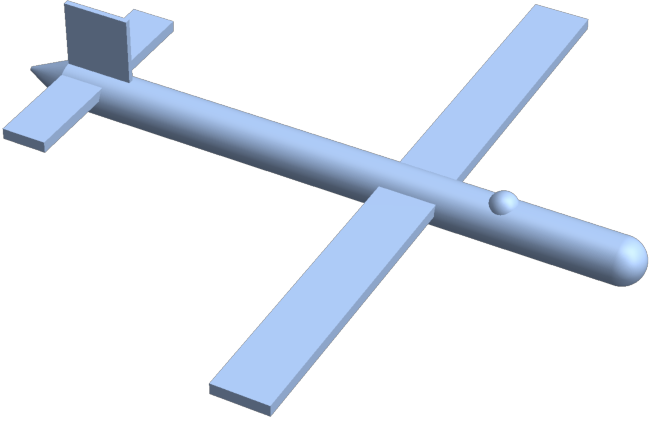
\includegraphics[ scale = 0.65 ]{\pLocalGraphics/b20/b20-glamor}
\end{frame}

\begin{frame}
	\frametitle{Defining the Spectrum}
	Let $\bl{\Omega_{P}}$, be a triangular partition of $\Omega$\\[10pt]
	\centering
	\raisebox{2cm}{$\bl{\Omega_{P}} = $} 
	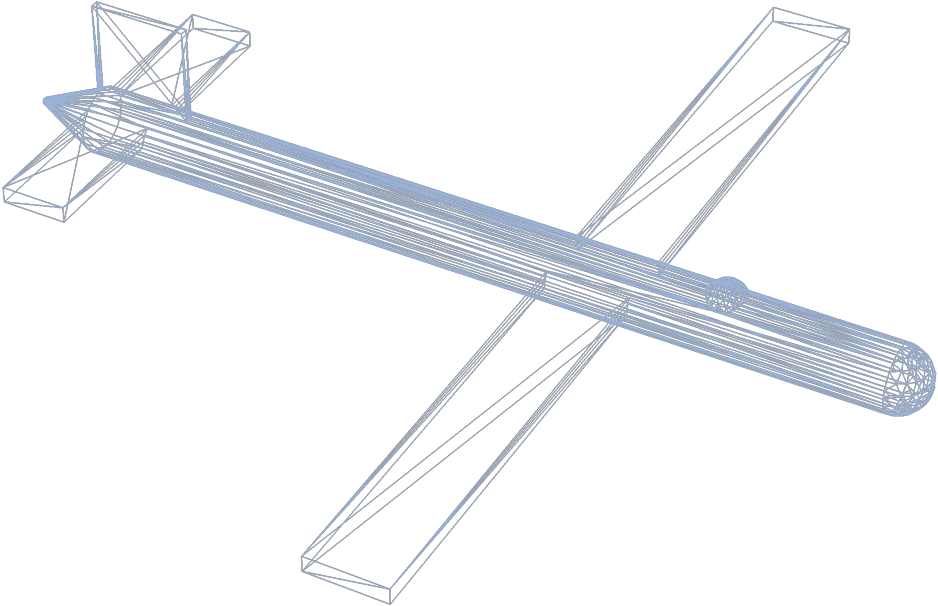
\includegraphics[ scale = 0.45 ]{\pLocalGraphics/b20/wire-1}
	\raisebox{2cm}{$= \bigcup\limits_{k=1}^{m}\tau_{k}$}
\end{frame}

\begin{frame}
	\frametitle{Defining the Spectrum}
	Properties of the triangular partition $\bl{\Omega_{P}}$\\[10pt]
	\begin{enumerate}
		\item $ \Omega_{P} = \bigcup\limits_{k=1}^{m}\tau_{k} $\\[10pt]
		\item $\text{Area}\paren{\Omega_{P}} = \text{Area}\paren{\bigcup_{k=1}^{m}\tau_{k}}$\\[10pt]
		\item $\text{Area}\paren{\tau_{k}} > 0, \quad k = 1:m$\\[10pt]
		\item $\tau_{k} \cap \tau_{j} = \delta_{k}^{j} \times$Area $\paren{\tau_{j}}$
	\end{enumerate}
\end{frame}

\begin{frame}
	\frametitle{Defining the Spectrum}
	Colloquially, it's a good mesh:\\[10pt]
	\begin{enumerate}
		\item The mesh is watertight (sealed)
		\item No triangles overlap
		\item No triangles underlap
	\end{enumerate}
\end{frame}

\begin{frame}
	\frametitle{Defining the Spectrum}
	Define $\alpha_{k}$ as the area of triangle $\tau_{k}$\\[10pt]
	\begin{enumerate}
		\item Define $\alpha_{k}$ as the area of triangle $\tau_{k}$
		\item The sequence is in ascending order:
		$$0 < \alpha_{1} \le \alpha_{2} \le \dots \le \alpha_{m}$$
 		\item The \bl{spectrum} is the sequence $\bl{\lst{\alpha_{k}}_{k=1}^{m}}$
	\end{enumerate}
\end{frame}

\begin{frame}
	\frametitle{Spectral Radius}
	Define $T$, the \bl{spectral radius} as\\[10pt]
	$$T=\ln \tau_{m} - \ln \tau_{1} = \ln \frac{\tau_{m}}{\tau_{1}}$$
\end{frame}

\begin{frame}
	\frametitle{Seeing the Spectral Radius}
	\begin{table}
		\begin{center}
			\begin{tabular}{ccc}
					%
				Mesh && \phantom{wi}Spectrum \\\hline
				\ \\
					%
				\includegraphics[ scale = 0.40 ]{\pLocalGraphics/b20/"views-B20-standard-1m"} &&
				\includegraphics[ scale = 0.35 ]{\pLocalGraphics/b20/"spectral-radius"} \\
					%
			\end{tabular}
		\end{center}
	\end{table}
	\centering
	Think of the \bl{height} of the gray box as the \bl{spectral radius}
\label{tab:rectangle}
\end{frame}

\begin{frame}
	\frametitle{Spectral Radius}
	Compare to $\kappa$ the \bl{matrix condition number} in the $2-$norm:\\[10pt]
	Given a matrix $\mathbf{A}$ of rank $\rho$ with singular value spectrum $\lst{\sigma_{k}}_{k=1}^{\rho}$\\
	The matrix condition number is defined as\\
	$$\kappa_{2} = \frac{\normt{\mathbf{A}}}{\normt{\mathbf{A}^{-1}}} = \bl{\frac{\sigma_{k}}{\sigma_{1}}}$$\\[10pt]
	$$T=\bl{\ln \frac{\tau_{m}}{\tau_{1}}}$$
\end{frame}

%     %     %     %     %     %     %     %     %
\subsection{What Works}

\begin{frame}
	\frametitle{Standard meshing, $1$ m resolution}
	\begin{table}[htp]
		\begin{center}
			\begin{tabular}{ccc}
					%
				Mesh && \phantom{wi}Spectrum \\\hline
				\ \\
					%
				\includegraphics[ scale = 0.40 ]{\pLocalGraphics b20/"views-B20-standard-1m"} &&
				\includegraphics[ scale = 0.35 ]{\pLocalGraphics b20/"dots-B20-standard-1m"} \\
					%
			\end{tabular}
		\end{center}
	\end{table}
\passed{}
\label{tab:standard-works-A}
\end{frame}

\begin{frame}
	\frametitle{Standard meshing, $0.1$ m resolution}
	\begin{table}[htp]
		\begin{center}
			\begin{tabular}{ccc}
					%
				Mesh && Spectrum \\\hline
				\ \\
					%
				\includegraphics[ scale = 0.40 ]{\pLocalGraphics b20/"views-B20-standard-0-1m"} &&
				\includegraphics[ scale = 0.35 ]{\pLocalGraphics b20/"dots-B20-standard-0-1m"} \\
					%
			\end{tabular}
		\end{center}
	\end{table}%
\passed{}
\label{tab:standard-works-B}
\end{frame}

\begin{frame}
	\frametitle{Standard meshing, $0.05$ m resolution}
	\begin{table}[htp]
		\begin{center}
			\begin{tabular}{ccc}
					%
				Mesh && Spectrum \\\hline
				\ \\
					%
				\includegraphics[ scale = 0.40 ]{\pLocalGraphics b20/"views-B20-standard-0-05m"} &&
				\includegraphics[ scale = 0.35 ]{\pLocalGraphics b20/"dots-B20-standard-0-05m"} \\
					%
			\end{tabular}
		\end{center}
	\end{table}%
\passed{}
\label{tab:standard-works-C}
\end{frame}

%     %     %     %     %     %     %     %     %
\subsection{What Doesn't Work}

\begin{frame}
	\frametitle{Standard meshing, $0.01$ m resolution}
	\begin{table}[htp]
		\begin{center}
			\begin{tabular}{ccc}
					%
				Mesh && Spectrum \\\hline
				\ \\
					%
				\includegraphics[ scale = 0.40 ]{\pLocalGraphics b20/"views-B20-standard-0-01m"} &&
				\includegraphics[ scale = 0.35 ]{\pLocalGraphics b20/"dots-B20-standard-0-01m"} \\
					%
			\end{tabular}
		\end{center}
	\end{table}%
	\tiny{\dg{\texttt{--------FATAL ERROR-------FATAL ERROR-------FATAL ERROR-------FATAL ERROR-------}}} \\
	\tiny{\dg{\texttt{ subroutine ACA\_Sum\_Update( A, S, Tol, RefNorm )  : }}\scrr{RHS: ACA did not converge}} \\
\tiny{\texttt{\dg{ = \phantom{---------}0}}}
\label{tab:features}
\end{frame}

\begin{frame}
	\frametitle{Standard meshing, $0.001$ m resolution}
	\begin{table}[htp]
		\begin{center}
			\begin{tabular}{ccc}
					%	r
				Mesh && Spectrum \\\hline
				\ \\
					%
				\includegraphics[ scale = 0.40 ]{\pLocalGraphics b20/"views-B20-standard-0-001m"} &&
				\includegraphics[ scale = 0.35 ]{\pLocalGraphics b20/"dots-B20-standard-0-001m"} \\
					%
			\end{tabular}
		\end{center}
	\end{table}%
	\tiny{\dg{\texttt{--------FATAL ERROR-------FATAL ERROR-------FATAL ERROR-------FATAL ERROR-------}}}\\
	\tiny{\dg{\texttt{subroutine Geometry\_TRI\_Compute( Tris, tol ) :}\scrr{Have Triangles with effective zero area}}}\\
	\tiny{\dg{\texttt{nTris\_With\_Zero\_Area = \phantom{--------}60}}}
\label{tab:features}
\end{frame}

\begin{frame}
	\frametitle{Mefisto meshing, $1$ m resolution}
	\begin{table}[htp]
		\begin{center}
			\begin{tabular}{ccc}
					%
				Mesh && Spectrum \\\hline
				\ \\
					%
				\includegraphics[ scale = 0.45 ]{\pLocalGraphics b20/"views-B20-mephisto-1-m"} &&
				\includegraphics[ scale = 0.40 ]{\pLocalGraphics b20/"dots-B20-mephisto-1-m"} \\
				%\put(-50,50) {\tiny{\rd{\texttt{--------FATAL ERROR-------FATAL ERROR-------FATAL ERROR-------FATAL ERROR-------}}}}
				%\put(-50,45) {\tiny{\rd{\texttt{ subroutine ACA\_Sum\_Update( A, S, Tol, RefNorm )  : RHS: ACA did not converge}}}}
					%
			\end{tabular}
		\end{center}
	\end{table}%
	\tiny{\dg{\texttt{--------FATAL ERROR-------FATAL ERROR-------FATAL ERROR-------FATAL ERROR-------}}} \\
	\tiny{\dg{\texttt{ subroutine ACA\_Sum\_Update( A, S, Tol, RefNorm )  : }}\scrr{RHS: ACA did not converge}} \\
\tiny{\texttt{\dg{ = \phantom{---------}0}}}
\label{tab:features}
\end{frame}

\begin{frame}
	\frametitle{Netgen meshing, {\it{very fine}} resolution}
	\begin{table}[htp]
		\begin{center}
			\begin{tabular}{ccc}
					%
				Mesh && Spectrum \\\hline
				\ \\
					%
				\includegraphics[ scale = 0.40 ]{\pLocalGraphics b20/"views-B20-netgen-very-fine"} &&
				\includegraphics[ scale = 0.35 ]{\pLocalGraphics b20/"dots-B20-netgen-very-fine"} \\
					%
			\end{tabular}
		\end{center}
	\end{table}%
%	\tiny{\dg{\texttt{--------FATAL ERROR-------FATAL ERROR-------FATAL ERROR-------FATAL ERROR-------}}} \\
%	\tiny{\dg{\texttt{ subroutine ACA\_Sum\_Update( A, S, Tol, RefNorm )  : }}\scrr{RHS: ACA did not converge}} \\
%	\tiny{\dg{\texttt{ =            0}}}
\tiny{\texttt{\dg{-------FATAL ERROR-------FATAL ERROR-------FATAL ERROR-------FATAL ERROR-------}}} \\
\tiny{\texttt{\dg{subroutine ACA\_Sum\_Update( A, S, Tol, RefNorm )  : }}\scrr{RHS: ACA did not converge}} \\
\tiny{\texttt{\dg{ = \phantom{---------}0}}}
\label{tab:features}
\end{frame}


\endinput  %  ==  ==  ==  ==  ==  ==  ==  ==  ==
